\documentclass[twocolumn, 11pt]{jsarticle}

\usepackage[utf8]{inputenc}
\usepackage[dvipdfmx]{graphicx}
\usepackage[top=25truemm, bottom=25truemm, left=20truemm, right=20truemm]{geometry}
\usepackage{okumacro}
\usepackage{amsmath, amssymb}
\usepackage{enumerate}
\usepackage{siunitx}
\usepackage{url}
\usepackage{pdfpages}
\usepackage{here}
\usepackage{diagbox}
\usepackage{slashbox}
\usepackage{svg}

\setcounter{secnumdepth}{6}
\setlength\textfloatsep{2truemm}

%---------------------------------------------------------------------

% \fontsize{11ptj}{16ptj}\selectfont
\setlength{\baselineskip}{16pt}
\setlength{\columnsep}{5mm}

%---------------------------------------------------------------------

%表
\usepackage{tabularx}
   \newcolumntype{C}{>{\centering\arraybackslash}X}
   \newcolumntype{L}{>{\raggedright\arraybackslash}X}
   \newcolumntype{R}{>{\raggedleft\arraybackslash}X}

%---------------------------------------------------------------------

\usepackage{listings,jvlisting}
\lstset{
    basicstyle={\ttfamily},
    identifierstyle={\small},
    commentstyle={\smallitshape},
    keywordstyle={\small\bfseries},
    ndkeywordstyle={\small},
    stringstyle={\small\ttfamily},
    frame={tb},
    tabsize=4,
    breaklines=true,
    columns=[l]{fullflexible},
    numbers=left,
    xrightmargin=0zw,
    xleftmargin=3zw,
    numberstyle={\scriptsize},
    stepnumber=1,
    numbersep=1zw,
    lineskip=-0.5ex
}
\newcommand{\prog}[3]{
    \lstinputlisting[label=code:#1, caption=#2]{figures/#3}
}
\renewcommand{\lstlistingname}{コード}

%---------------------------------------------------------------------
\makeatletter
\def\Hline{
    \noalign{\ifnum0=`}\fi\hrule \@height 2pt \futurelet
    \reserved@a\@xhline
}
\makeatother

%キャプション(番号無し)
\newcommand{\subcaption}[1]{
    #1 \\
    \vskip\baselineskip
}

%表の空欄
\newcommand{\blank}{\textbf{---}}

%数式(番号付き)
\newcommand{\eq}[1]{
    \begin{eqnarray}
        #1
    \end{eqnarray}
}
%数式(番号無し)
\newcommand{\EQ}[1]{
    \begin{eqnarray*}
        #1
    \end{eqnarray*}
}

%一階微分
\newcommand{\diff}[2]{\frac{d #1}{d #2}}
%二階微分
\newcommand{\DIFF}[2]{\frac{d^2 #1}{d {#2}^2}}

%図(1つ)
\newcommand{\fig}[4][0.9]{
    \begin{figure}[H]
        \centering
        \includegraphics[width=#1\linewidth]{figures/#2}
        \caption{#3}
        \label{fig:#4}
    \end{figure}
}
%図(2つ)
\newcommand{\ffig}[6]{
    \begin{figure}[H]
        \centering
        \begin{minipage}{0.45\linewidth}
            \centering
            \includegraphics[width=\linewidth]{figures/#1}
            \caption{#2}
            \label{fig:#3}
        \end{minipage}
        \begin{minipage}{0.45\linewidth}
            \centering
            \includegraphics[width=\linewidth]{figures/#4}
            \caption{#5}
            \label{fig:#6}
        \end{minipage}
    \end{figure}
}
%図(3つ)
\newcommand{\fffig}[9]{
    \begin{figure}[H]
        \begin{minipage}{0.3\linewidth}
            \centering
            \includegraphics[width=\linewidth]{figures/#1}
            \caption{#2}
            \label{fig:#3}
        \end{minipage}
        \begin{minipage}{0.3\linewidth}
            \centering
            \includegraphics[width=\linewidth]{figures/#4}
            \caption{#5}
            \label{fig:#6}
        \end{minipage}
        \begin{minipage}{0.3\linewidth}
            \centering
            \includegraphics[width=\linewidth]{figures/#7}
            \caption{#8}
            \label{fig:#9}
        \end{minipage}
    \end{figure}
}
% %svg(1)
% \newcommand{\svg}[4][0.9]{
%     \begin{figure}[H]
%         \centering
%         \includesvg[width=#1\linewidth]{figures/#2}
%         \caption{#3}
%         \label{fig:#4}
%     \end{figure}
% }
% %svg(2)
% \newcommand{\ssvg}[6]{
%     \begin{figure}[H]
%         \centering
%         \begin{minipage}{0.45\linewidth}
%             \centering
%             \includesvg[width=\linewidth]{figures/#1}
%             \caption{#2}
%             \label{fig:#3}
%         \end{minipage}
%         \begin{minipage}{0.45\linewidth}
%             \centering
%             \includesvg[width=\linewidth]{figures/#4}
%             \caption{#5}
%             \label{fig:#6}
%         \end{minipage}
%     \end{figure}
% }
% %svg(3)
% \newcommand{\sssvg}[9]{
%     \begin{figure}[H]
%         \begin{minipage}{0.3\linewidth}
%             \centering
%             \includesvg[width=\linewidth]{figures/#1}
%             \caption{#2}
%             \label{fig:#3}
%         \end{minipage}
%         \begin{minipage}{0.3\linewidth}
%             \centering
%             \includesvg[width=\linewidth]{figures/#4}
%             \caption{#5}
%             \label{fig:#6}
%         \end{minipage}
%         \begin{minipage}{0.3\linewidth}
%             \centering
%             \includesvg[width=\linewidth]{figures/#7}
%             \caption{#8}
%             \label{fig:#9}
%         \end{minipage}
%     \end{figure}
% }
\pagestyle{empty}

\begin{document} 

\twocolumn[
    \centering
    {\LARGE \textbf{2-コーダルリング$CR(N, 4, *)$の独立全域木の構築}}\\
    \vspace{1zw}
    {\large E1832 藤村勇仁 \hspace{3zw} 指導教員 濱田幸弘}\\
    \vspace{2zw}
]

\section{はじめに}
    グラフ理論とは、ネットワークや交通などの様々な問題をグラフを用いて表現することで、グラフの持つ性質から解析を行う分野である。本研究ではグラフ理論をデータ通信に関する問題を解決するために用いる。
    グラフの2頂点間に内素な道がn本あれば、n-1本の道が故障しても通信が行うことができる。また、データを分割して冗長性を持たせて送信することで、いくつかのデータが破損や送信失敗した場合でも受信者側でデータの復元を行うことができる。
    本研究では、このような問題を解決するために2-コーダルリングというグラフ上での独立全域木の構築について述べる。

\section{グラフ}
    \subsection{グラフ}
        グラフ$G$は頂点の空でない有限集合$V(G)$(頂点集合)と、$V(G)$の二要素部分集合である辺の集合$E(G)$(辺集合)のことであり、このようなグラフを$G=(V,E)$と書く。また、頂点の数を位数、辺の数をサイズといい、位数$p$、サイズ$q$のグラフを$(p,q)$グラフという。\cite{2006離散数学入門}

    \subsection{道}
        $(v_{i-1}, v_i) \in E$を満たす頂点の列$P = \langle v_0, v_1, \cdots, v_n \rangle$を道といい、$n$を$P$の長さという。$v_0$を$P$の始点, $v_n$を$P$の終点といい、$v_0 = v_n$のとき$P$は閉路という。\cite{2006離散数学入門}

    \subsection{内素}
        複数の道が内素であるとは、始点と終点を接続する辺から成る道が高々1つで、どの2つの道も始点と終点以外で同じ頂点を通っていないことをいう。\cite{chartrand1993applied}
    
    \subsection{木}
        どの2頂点間にも道が存在し、閉路を含まないグラフを木という。

    \subsection{全域木}
        連結グラフ$G$の全域部分グラフ$G'$が木であるなら、$G'$のことを全域木と呼ぶ。\cite{2006離散数学入門}

    \subsection{独立全域木}
        グラフ$G$において同一の頂点を根としている2個の全域木について、根を始点とし根を除く任意の頂点を終点とする道が内素であるとき、これらの全域木は独立であるという。\cite{chartrand1993applied}

    \subsection{2-コーダルリング}
        2-コーダルリングは、次のように定義され、$CR(N, d_1, d_2)$と書かれる。\cite{YukihiroHAMADA2016}
        \begin{equation*}
            \begin{split}
                G &= (V, E) \\
                V &= \{0, 1, \cdots, N-1\} \\
                E &= \{(u, v) \mid [v-u]_N = 1 \text{or} [v-u]_N = d_i, \\
                  &\qquad 1 \geqq i \geqq 2, 2 \geqq d_1 < d_2 \geqq N/2\} \\
                  &\text{ここで、}[v-u]_N \text{は} (v-u) \bmod N \text{を示す}
            \end{split}
        \end{equation*}
        2-コーダルリングは、$N\geq7, d_2\neq\frac{N}{2}$のとき$CR(N,d_1,d_2)$は6-正則であるという性質を持つ。
        図\ref{fig:chordal}に$N = 14, d_1 = 4, d_2 = 7$の2-コーダルリングを、図\ref{fig:IST}にその2-コーダルリング上の同じ頂点を根とする二つの独立全域木を示す。
      
        \fig[0.7]{chordal.pdf}{$CR(14,4,7)$}{chordal}
        \begin{figure}[H]
            \centering
            \begin{minipage}{0.45\linewidth}
                \centering
                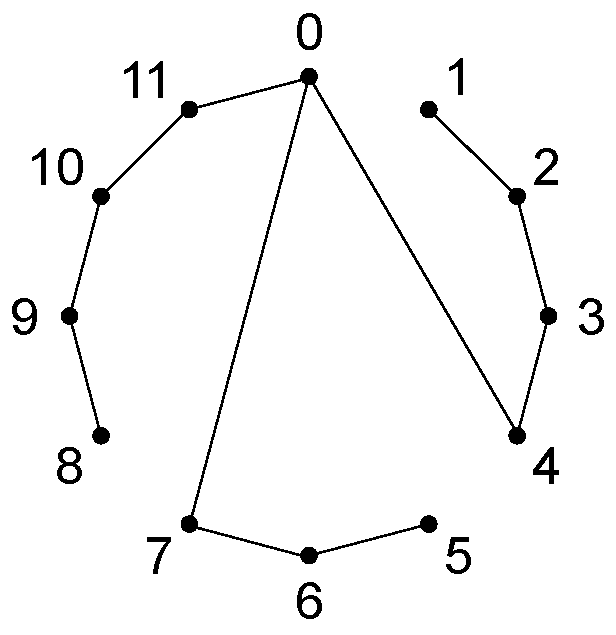
\includegraphics[width=\linewidth]{figures/IST1.pdf}
            \end{minipage}
            \begin{minipage}{0.45\linewidth}
                \centering
                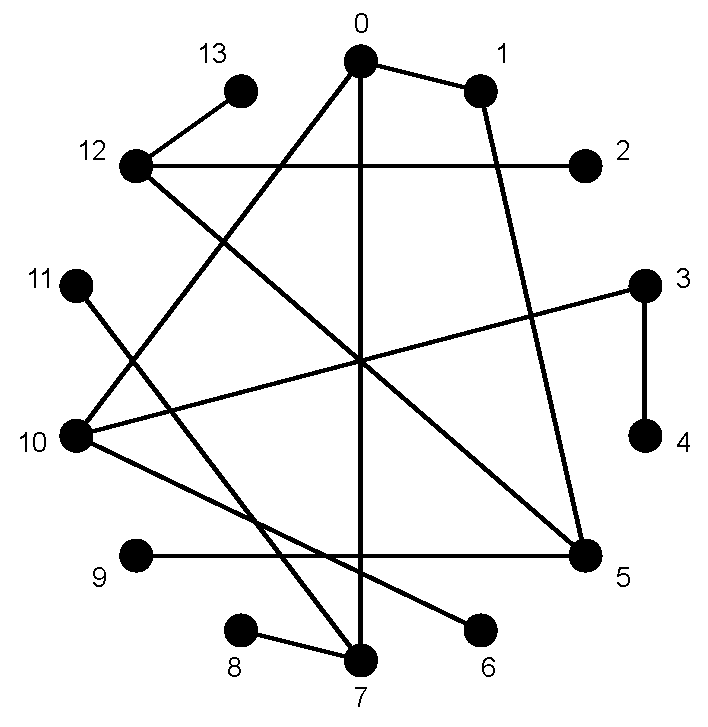
\includegraphics[width=\linewidth]{figures/IST2.pdf}
            \end{minipage}
            \caption{$CR(14,4,7)$の二つの独立全域木}
            \label{fig:IST}
        \end{figure}

\section{本研究について}
    \subsection{先行研究}
        先行研究により、以下が知られている。
        \begin{itemize}
            \item グラフがk-連結であることと、グラフの任意の2頂点間に少なくともk本の内素な道が存在することが同値である。 \cite{YukihiroHAMADA2016} それにより、2-コーダルリングについても同様にk-連結であればk本の内素な道が存在するが、具体的な構築方法は2-コーダルリングの多くで知られていない。
            \item 以下に示す6連結のコーダルリング$CR(N,d_1,d_2)$において6つの全域木を構築するアルゴリズムが考案され、それらが独立であることがプログラムを使い検証されている。\cite{Yokooji}
                \begin{itemize}
                    \item $N\geqq7, d_1=2, d_2=3$
                    \item $N\geqq4n+1(n\geqq2), d_1=2, d_2=4$
                    \item $N\geqq10, d_12=, d_2=4$
                    \item $N\geqq13, d_1=2, d_2=5$
                    \item $N\geqq3d_2-2, d_1=2, 2<d_2=N/2$
                    \item $N\geqq9, d_1=3, d_2=4$
                    \item $N\geqq17, 3\leqq d_1\leqq\frac{N-1}{4}=, d_2=2d_1-1$
                    \item $N\geqq10, 2\leqq d_1\leqq\frac{N}{5}, d_2=2d_1$
                    \item $N\geqq9, 2\leqq d_1\leqq\frac{N}{4}, d_2=2d_1$
                    \item $N\geqq5, 2\leqq d_1\leqq\frac{N-1}{3}, d_2=d_1+1$
                \end{itemize}
        \end{itemize}
        
    \subsection{目的}
        2-コーダルリング$CR(N, 4, *)$において、6つの全域木を構築するアルゴリズムを考案し、それらが独立であることをプログラムを使い検証することが本研究の目的である。$*$は4より大きく、$N/2$より小さい任意の整数を表す。これは、先行研究によりわかっていることより、これまでで開拓されていない値での2-コーダルリングに対して研究を行うためであり、6個の独立全域木が存在することはグラフが6連結であるということと同値であり、そのためには$*\neq\frac{N}{2}$である必要があるからである。

    \subsection{進捗}
        4年の課題研究、及び5年に入ってからの半年間でグラフ理論に関する資料や先行研究者の論文を読んで研究対象に関する知識を身に着けた。

\section{今後の方針}
    目的で述べたように、最終的には2-コーダルリング$CR(N,4,*)$上で全域木を6個構築し、独立かどうかを検証する。そのために、2-コーダルリング$CR(N,4,*)$上で6つの全域木を構築するアルゴリズムを考案し、それが独立であるかをプログラムを作成し検証する。
    
    
\bibliographystyle{jplain}
\bibliography{reference.bib}

\end{document}
